\documentclass[12]{article}%12pt即为*四号字
\usepackage{ctex}%引入中文包
\usepackage{graphicx}%插入图片的包
\usepackage{geometry}%设置A4纸页边距的包
\usepackage{url}
\usepackage{stfloats}
\usepackage{float}
\usepackage{amssymb}
\geometry{left=3.18cm,right=3.18cm,top=2.54cm,bottom=2.54cm}%设置页边距
\linespread{1}%设置行间距



\begin{document}
\begin{center}
    \LARGE\songti\textbf{微分方程数值解Project1作业报告} \\%标题
    \large\kaishu\textbf{褚朱钇恒\qquad 3200104144}%一般是我的姓名
\end{center}
\section{运行说明}
    本项目需要调用\verb|jsoncpp|与\verb|eigen3|库,故请在运行此项目前安装好这两个包。

    在\verb|project|目录下使用\verb|make|命令即可编译整个项目并得到实验报告。

\section{程序设计思路}
所有实现样条计算的相关代码都在头文件\verb|BVP.h|中,其中设计了一下几个类:
\subsection{Class Function}
其定义了\verb|()|,\verb|diff_x|,\verb|diff2_x|,\verb|diff_y|,\verb|diff2_y|,\verb|laplace|六个虚函数,分别用于函数求值,求导,求二阶导和求拉普拉斯算子。

\subsection{Class point}
定义了平面上的向量运算和求向量长度。

\subsection{Class Circle}
定义了圆与直线的求交算法


\subsection{Class FD\_Methods}
有限差分法的虚类,定义了\verb|solve|,\verb|()|,\verb|error_norm|三个虚函数,分别用于求解,求值和求误差的范数。该基类有以下两个派生类:
\begin{itemize}
    \item FD\_regular 使用有限差分法在单位正方形上进行微分方程的求解
    \item FD\_irregular 使用有限差分法在单位正方形内部去掉一个圆的区域上进行微分方程的求解 
\end{itemize}
两者都可以输入以下参数:
\begin{itemize}
    \item \verb|h|:网格粗细
    \item \verb|f|:计算的微分方程的真实解
    \item \verb|cond|:边值条件(1表示Dirichlet,2表示Neumann,3表示混合条件)
\end{itemize}
FD\_irregular则需要一个额外的参数C,表示去掉的圆的区域。

\section{程序测试结果}
我选择的测试用的函数为:
\begin{itemize}
    \item $f(x,y)=e^{x+sin(y)}$
    \item $f(x,y)=sin(3x+3y)$
    \item $f(x,y)=e^(x^3+y^3)$
\end{itemize}

\subsection{整体效果}
由于单位正方形上的图像比较方便绘制,所以这里展示部分单位正方形上的求解结果。

对第一个函数$f(x,y)=e^{x+sin(y)}$使用Dirichlet边值条件求解,结果如下:
\begin{figure}[H]
    \centering
    \begin{minipage}[t]{0.48\textwidth}
    \centering
    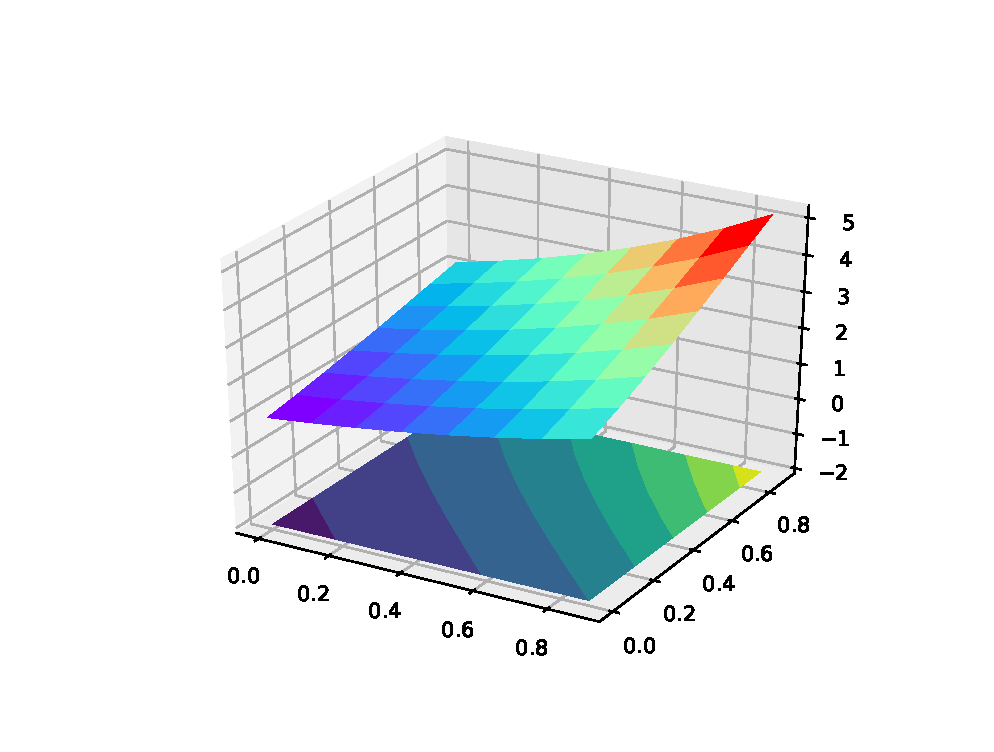
\includegraphics[width=6cm]{../pic/fun18.eps}
    \caption{n=8}
    \end{minipage}
    \begin{minipage}[t]{0.48\textwidth}
    \centering
    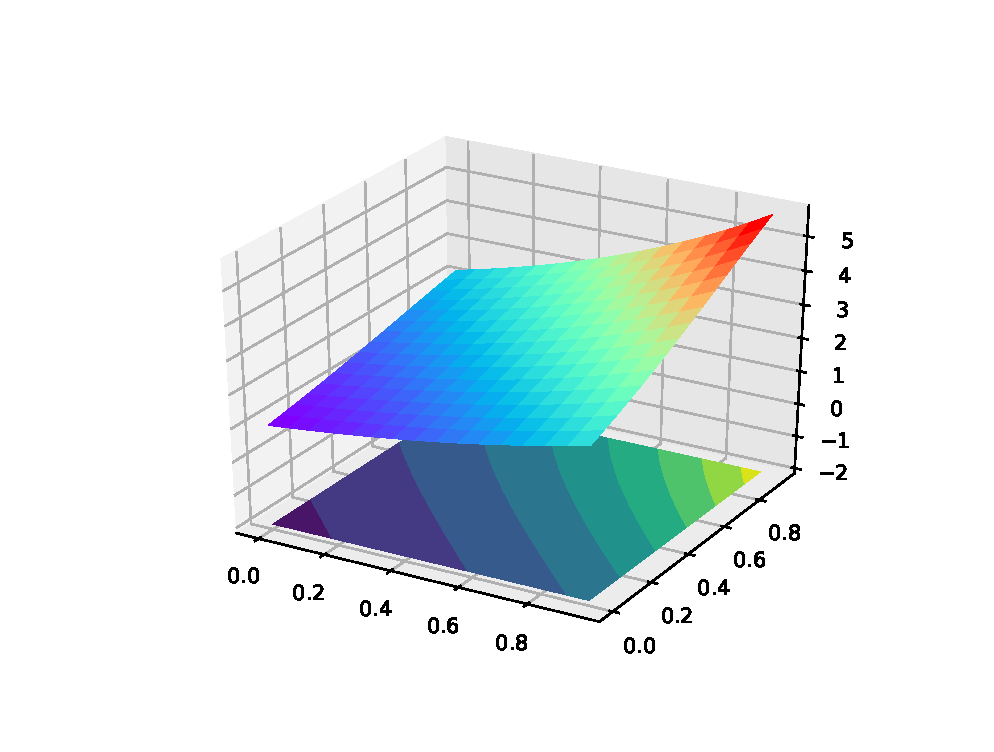
\includegraphics[width=6cm]{../pic/fun116.eps}
    \caption{n=16}
    \end{minipage}
\end{figure}
\begin{figure}[H]
    \centering
    \begin{minipage}[t]{0.3\textwidth}
    \centering
    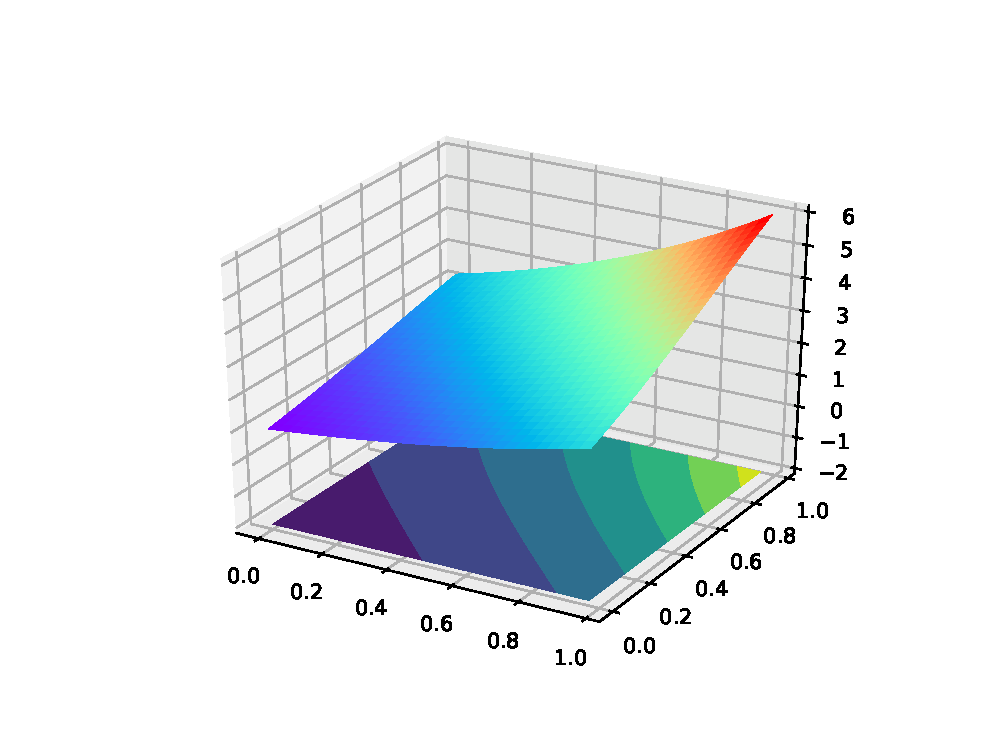
\includegraphics[width=5cm]{../pic/fun132.eps}
    \caption{n=32}
    \end{minipage}
    \begin{minipage}[t]{0.3\textwidth}
    \centering
    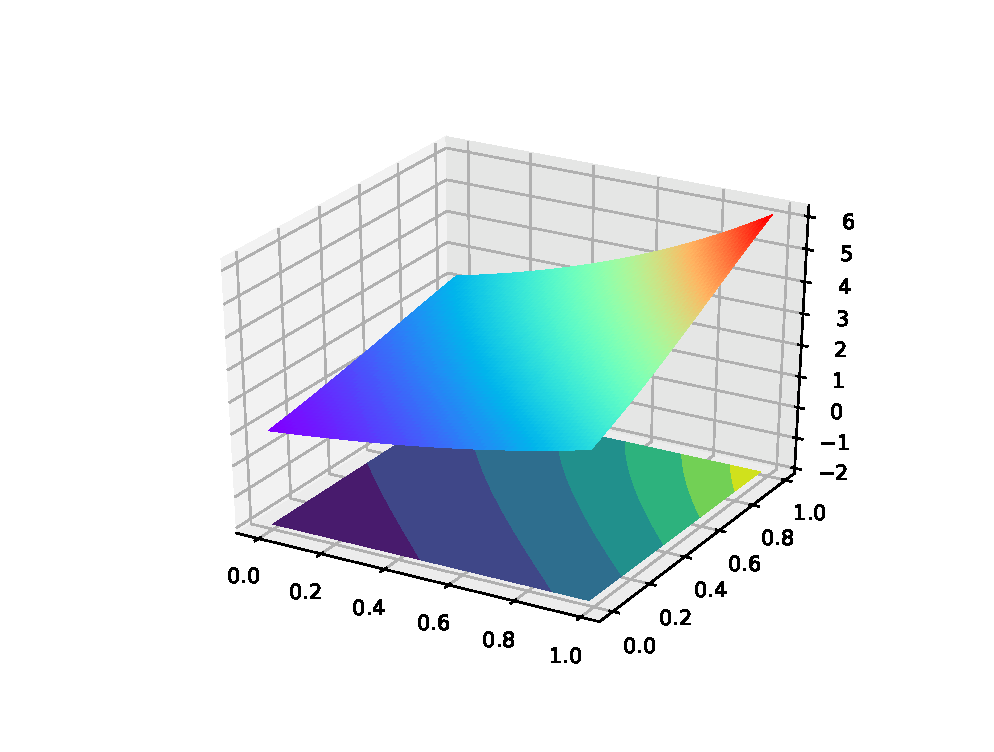
\includegraphics[width=5cm]{../pic/fun164.eps}
    \caption{n=64}
    \end{minipage}
    \begin{minipage}[t]{0.3\textwidth}
    \centering
    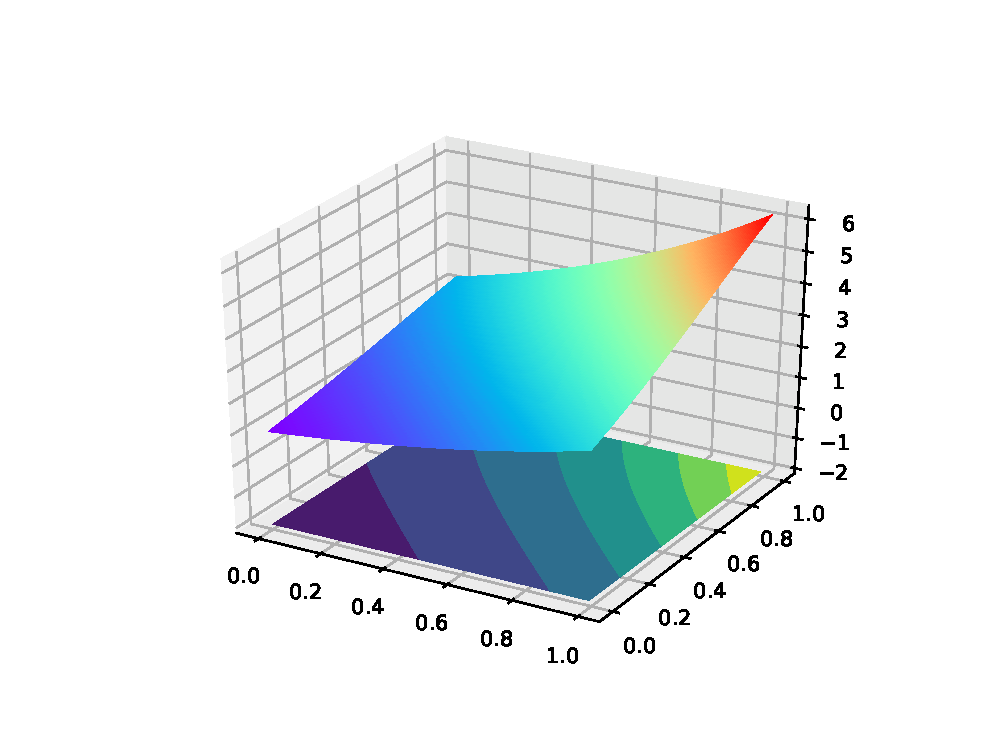
\includegraphics[width=5cm]{../pic/fun1128.eps}
    \caption{n=128}
    \end{minipage}
\end{figure}
    
对第二个函数$f(x,y)=sin(3x+3y)$使用Neumann边值条件求解,结果如下:
\begin{figure}[H]
    \centering
    \begin{minipage}[t]{0.48\textwidth}
    \centering
    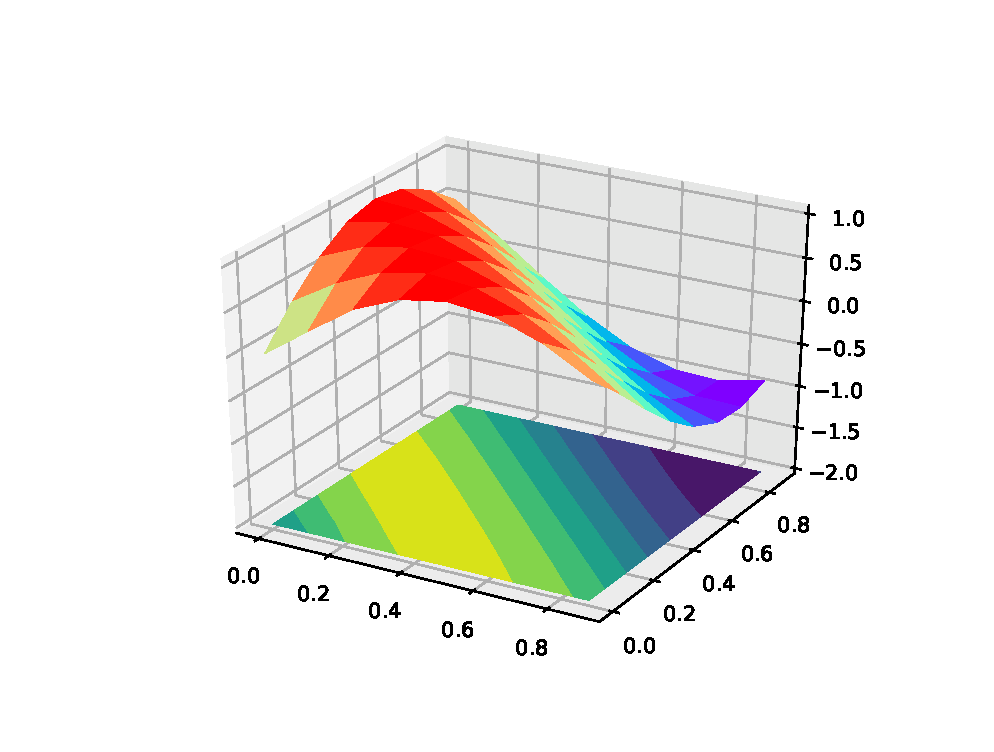
\includegraphics[width=6cm]{../pic/fun28.eps}
    \caption{n=8}
    \end{minipage}
    \begin{minipage}[t]{0.48\textwidth}
    \centering
    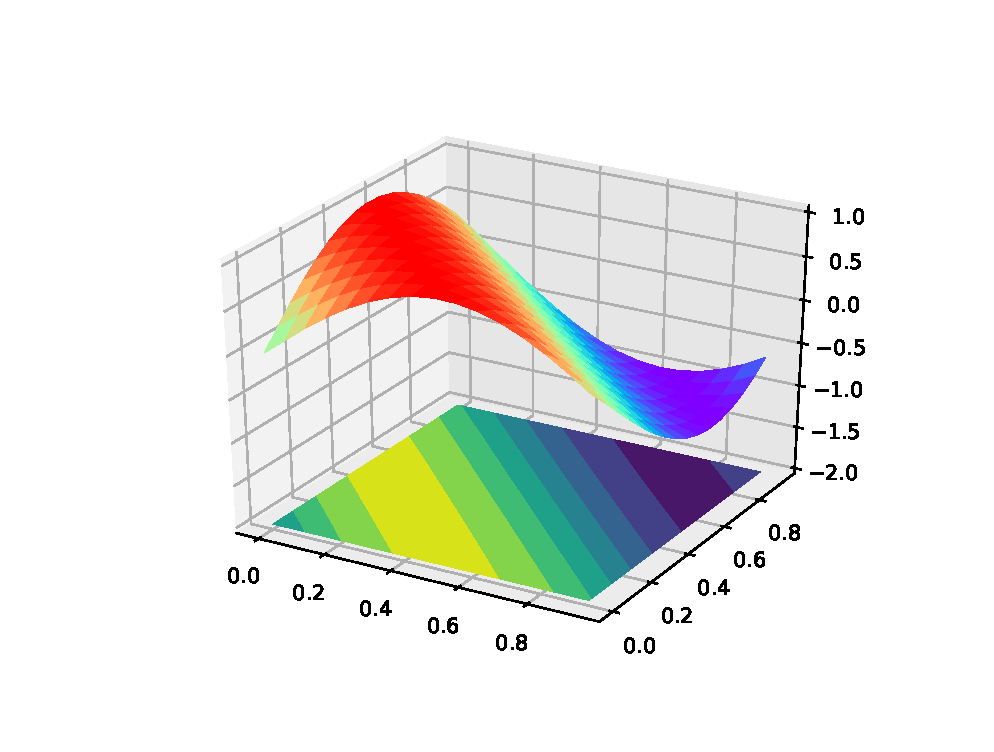
\includegraphics[width=6cm]{../pic/fun216.eps}
    \caption{n=16}
    \end{minipage}
\end{figure}
\begin{figure}[H]
    \centering
    \begin{minipage}[t]{0.3\textwidth}
    \centering
    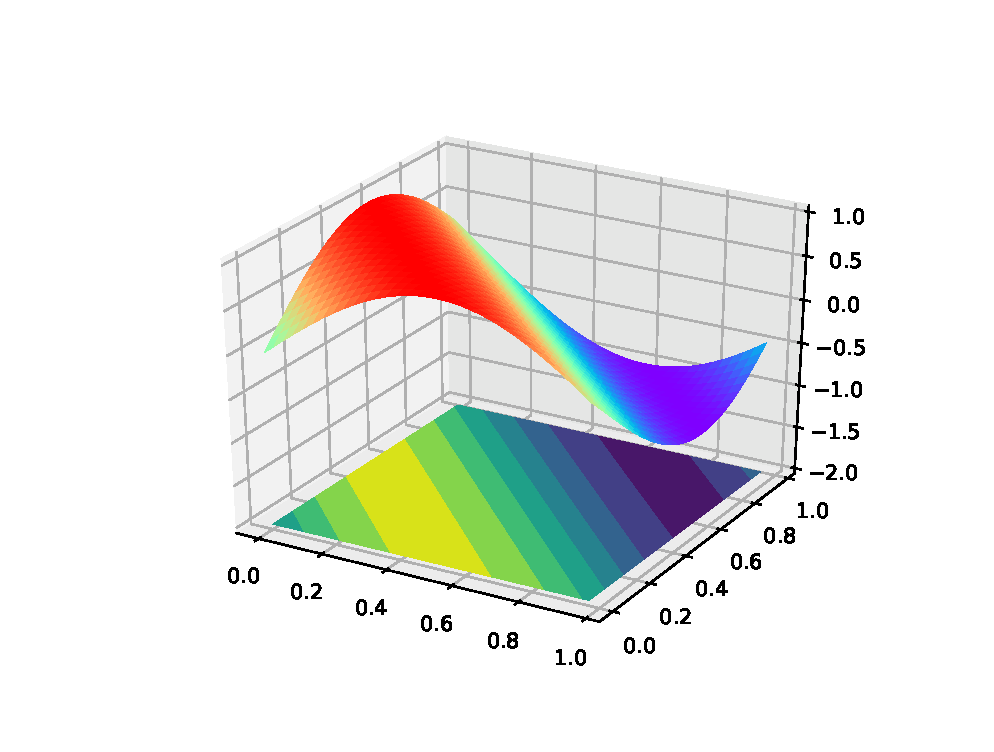
\includegraphics[width=5cm]{../pic/fun232.eps}
    \caption{n=32}
    \end{minipage}
    \begin{minipage}[t]{0.3\textwidth}
    \centering
    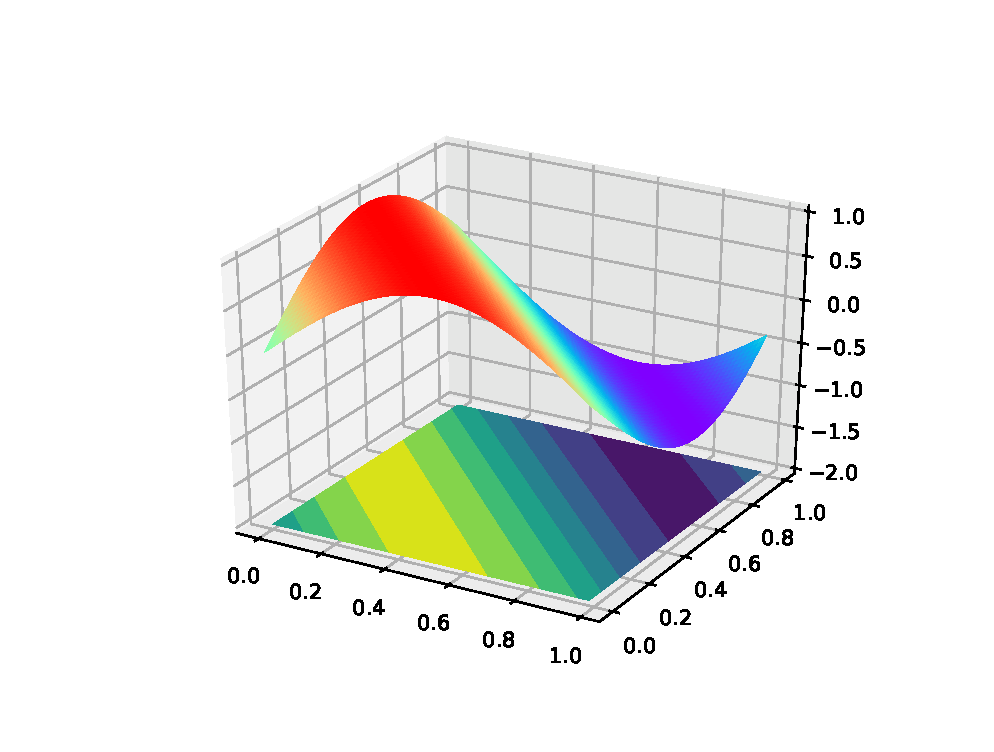
\includegraphics[width=5cm]{../pic/fun264.eps}
    \caption{n=64}
    \end{minipage}
    \begin{minipage}[t]{0.3\textwidth}
    \centering
    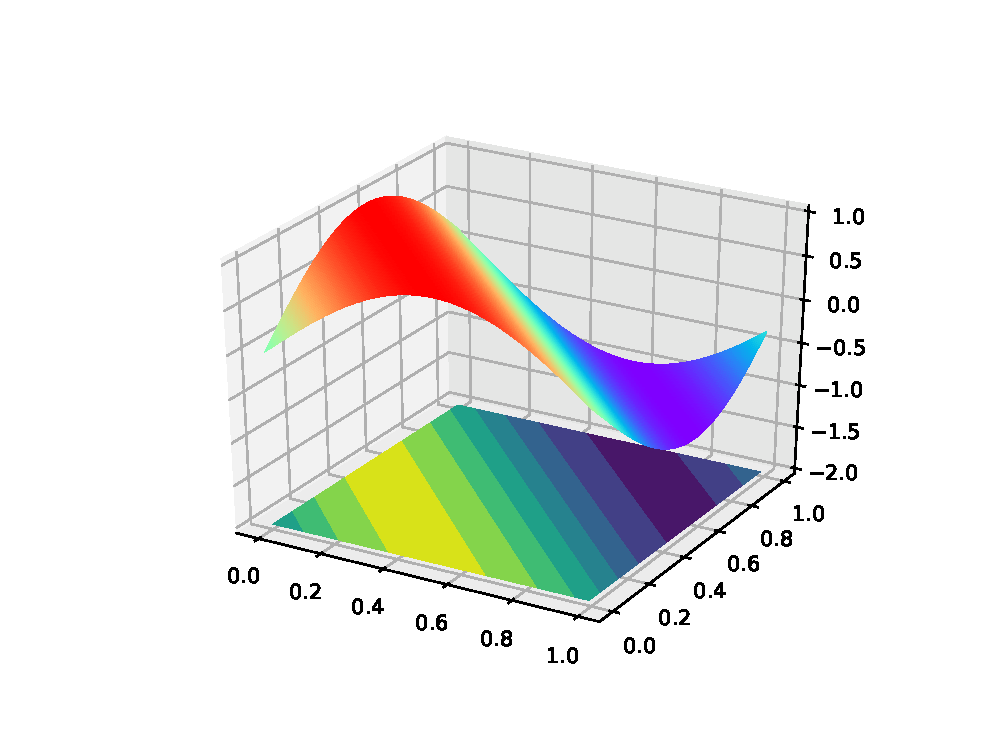
\includegraphics[width=5cm]{../pic/fun2128.eps}
    \caption{n=128}
    \end{minipage}
\end{figure}
对第三个函数$f(x,y)=e^(x^3+y^3)$使用混合边值条件(一条边Neumann边值条件,三条边Dirichlet边值条件)求解,结果如下:
\begin{figure}[H]
    \centering
    \begin{minipage}[t]{0.48\textwidth}
    \centering
    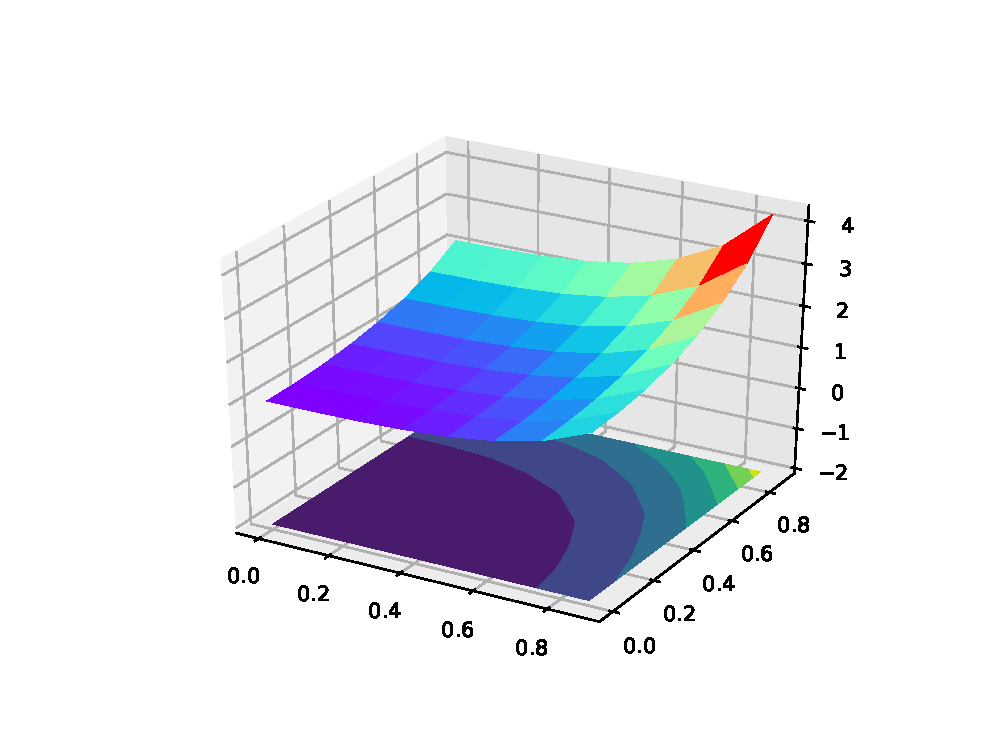
\includegraphics[width=6cm]{../pic/fun38.eps}
    \caption{n=8}
    \end{minipage}
    \begin{minipage}[t]{0.48\textwidth}
    \centering
    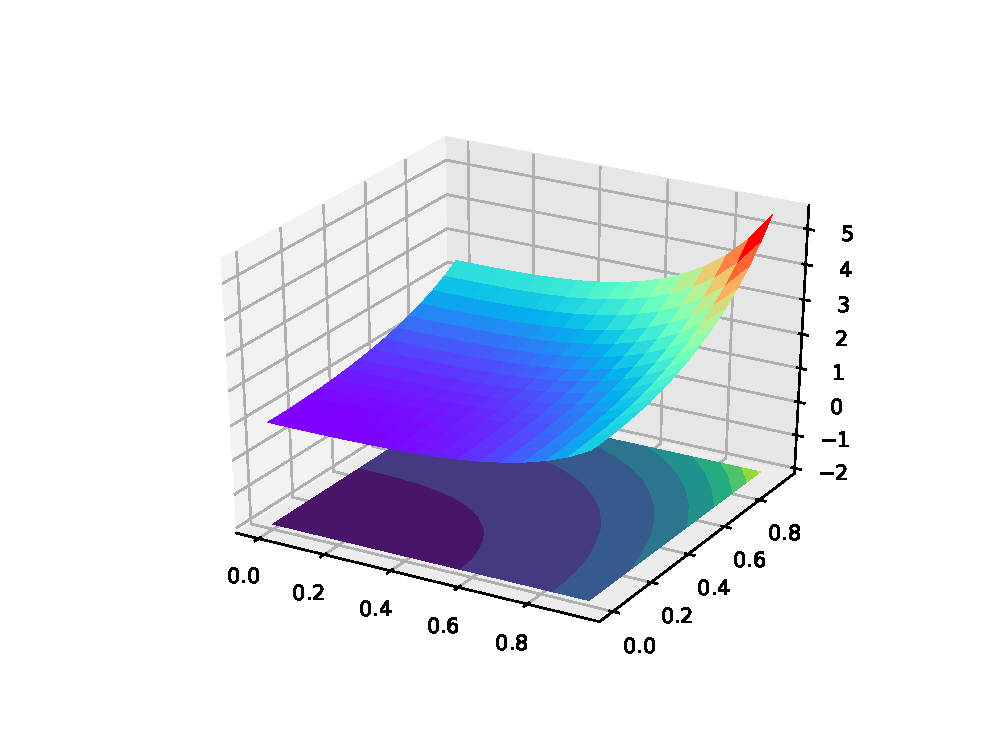
\includegraphics[width=6cm]{../pic/fun316.eps}
    \caption{n=16}
    \end{minipage}
\end{figure}
\begin{figure}[H]
    \centering
    \begin{minipage}[t]{0.3\textwidth}
    \centering
    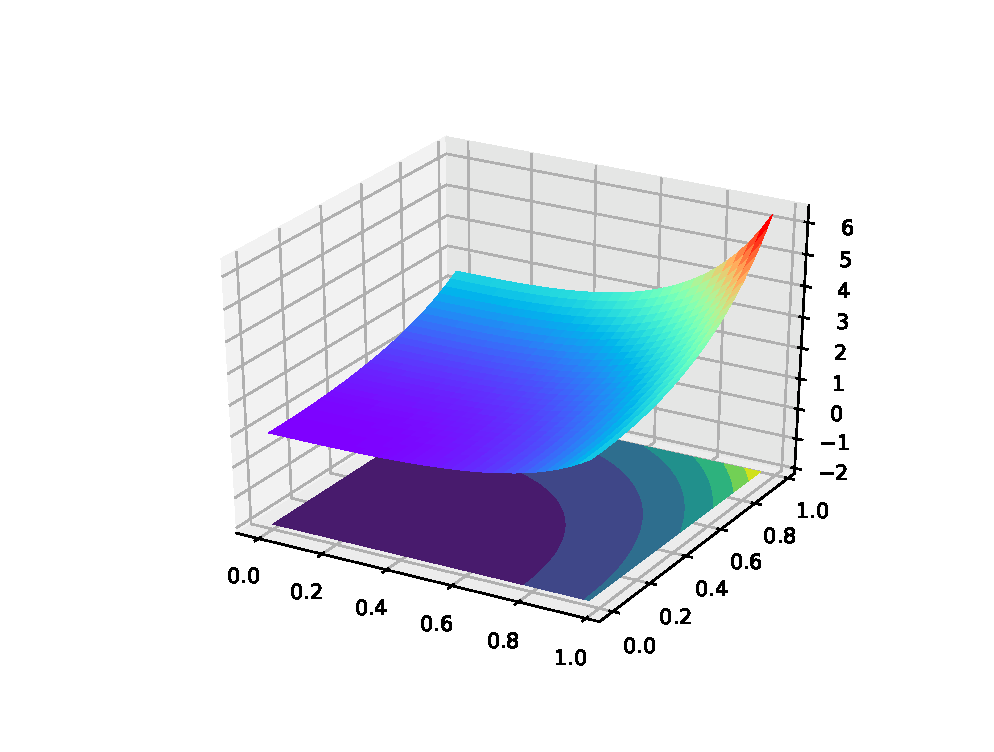
\includegraphics[width=5cm]{../pic/fun332.eps}
    \caption{n=32}
    \end{minipage}
    \begin{minipage}[t]{0.3\textwidth}
    \centering
    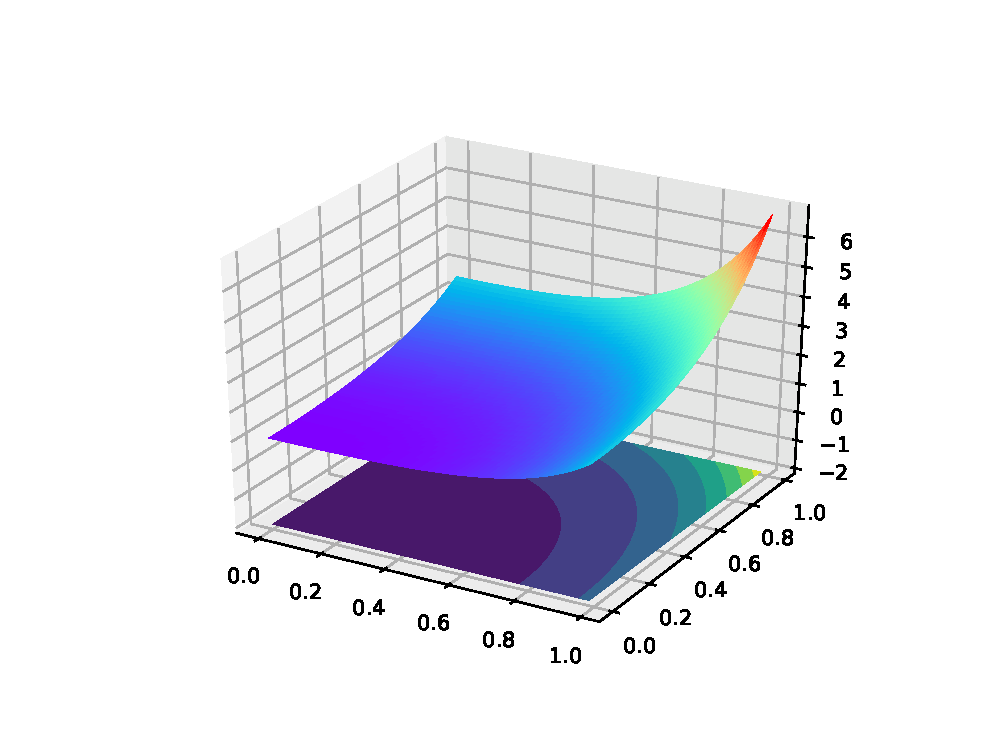
\includegraphics[width=5cm]{../pic/fun364.eps}
    \caption{n=64}
    \end{minipage}
    \begin{minipage}[t]{0.3\textwidth}
    \centering
    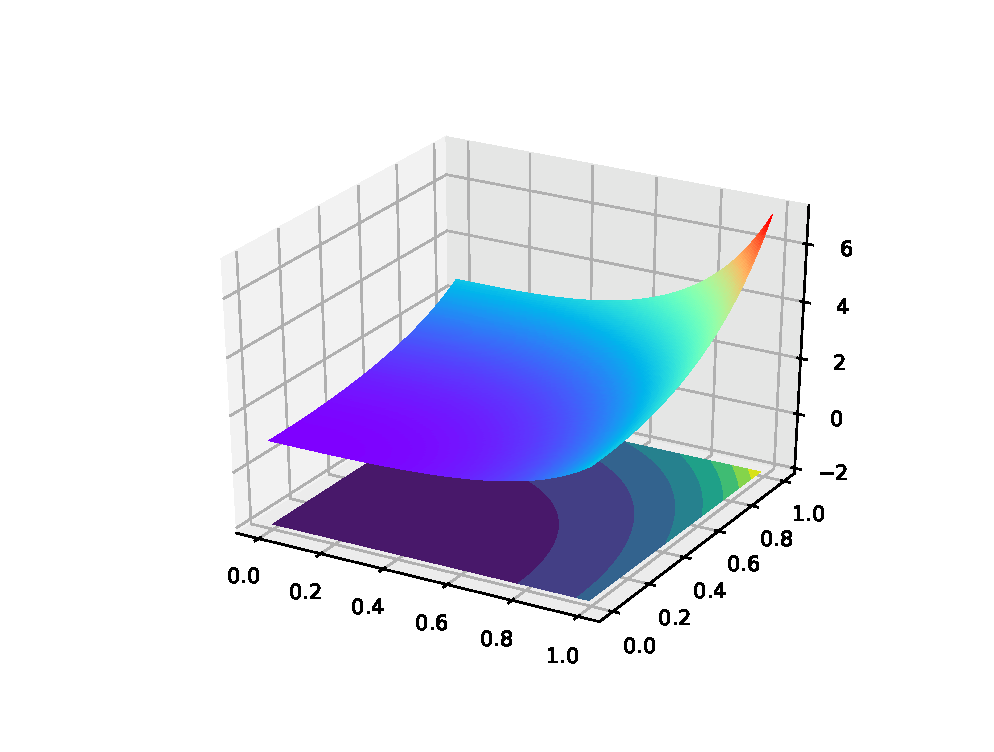
\includegraphics[width=5cm]{../pic/fun3128.eps}
    \caption{n=128}
    \end{minipage}
\end{figure}
\subsection{固定点收敛速率}
我们取$(0.25,0.25),(0.25,0.75),(0.75,0.25),(0.75,0.75)$四个固定点,计算他们的平均误差,加细网格计算其误差变小的速率。结果如下:

对于正则化区域,效果如下:
\begin{figure}[H]
    \centering
    \begin{minipage}[t]{0.3\textwidth}
    \centering
    \includegraphics[width=5cm]{../pic/fun1_regu_points.eps}
    \caption{$f(x,y)=e^(x^3+y^3)$}
    \end{minipage}
    \begin{minipage}[t]{0.3\textwidth}
    \centering
    \includegraphics[width=5cm]{../pic/fun2_regu_points.eps}
    \caption{$f(x,y)=sin(3x+3y)$}
    \end{minipage}
    \begin{minipage}[t]{0.3\textwidth}
    \centering
    \includegraphics[width=5cm]{../pic/fun3_regu_points.eps}
    \caption{$f(x,y)=e^(x^3+y^3)$}
    \end{minipage}
\end{figure}
基本可以认为三个方程中三个边值条件的固定点误差收敛速度关于h都是2阶的,但可能由于纯Neumann条件给出的系数矩阵的条件数较大,导致了算法的不稳定性变大,其收敛的速度明显小于另外两个条件。

对于非正则化区域,我们设挖去的圆形圆心为$(0.5,0.5)$,半径为$r=0.2$,效果如下(由于纯Neumann条件的代码尚未完成,缺少对圆上的Neumann条件的处理,所以此处只有两条曲线):
\begin{figure}[H]
    \centering
    \begin{minipage}[t]{0.3\textwidth}
    \centering
    \includegraphics[width=5cm]{../pic/fun1_irregu_points.eps}
    \caption{$f(x,y)=e^(x^3+y^3)$}
    \end{minipage}
    \begin{minipage}[t]{0.3\textwidth}
    \centering
    \includegraphics[width=5cm]{../pic/fun2_irregu_points.eps}
    \caption{$f(x,y)=sin(3x+3y)$}
    \end{minipage}
    \begin{minipage}[t]{0.3\textwidth}
    \centering
    \includegraphics[width=5cm]{../pic/fun3_irregu_points.eps}
    \caption{$f(x,y)=e^(x^3+y^3)$}
    \end{minipage}
\end{figure}
从整体趋势来看,收敛速度应该也是二阶的,但在误差比较大,可能是对于圆附近的ghost点的处理不太优美(目前的处理办法是在与坐标轴平行一个方向上找一个网格上的点,再圆上的点与网格上的点的值线性差值得到ghost点的约束条件)。

\subsection{误差范数及其收敛分析}

\subsubsection{正则化区域上的结果}
分别对三个方程使用Dirichlet,Neumann,mix条件求解,其误差范数收敛速度如下:
\begin{figure}[H]
    \centering
    \begin{minipage}[t]{0.3\textwidth}
    \centering
    \includegraphics[width=5cm]{../pic/fun1_regu_error_norm.eps}
    \caption{$f(x,y)=e^(x^3+y^3)$}
    \end{minipage}
    \begin{minipage}[t]{0.3\textwidth}
    \centering
    \includegraphics[width=5cm]{../pic/fun2_regu_error_norm.eps}
    \caption{$f(x,y)=sin(3x+3y)$}
    \end{minipage}
    \begin{minipage}[t]{0.3\textwidth}
    \centering
    \includegraphics[width=5cm]{../pic/fun3_regu_error_norm.eps}
    \caption{$f(x,y)=e^(x^3+y^3)$}
    \end{minipage}
\end{figure}
\subsubsection{非正则化区域上的结果}
分别对三个方程使用mix条件求解,其误差范数收敛速度如下:
\begin{figure}[H]
    \centering
    \begin{minipage}[t]{0.3\textwidth}
    \centering
    \includegraphics[width=5cm]{../pic/fun1_irregu_error_norm.eps}
    \caption{$f(x,y)=e^(x^3+y^3)$}
    \end{minipage}
    \begin{minipage}[t]{0.3\textwidth}
    \centering
    \includegraphics[width=5cm]{../pic/fun2_irregu_error_norm.eps}
    \caption{$f(x,y)=sin(3x+3y)$}
    \end{minipage}
    \begin{minipage}[t]{0.3\textwidth}
    \centering
    \includegraphics[width=5cm]{../pic/fun3_irregu_error_norm.eps}
    \caption{$f(x,y)=e^(x^3+y^3)$}
    \end{minipage}
\end{figure}
发现收敛速度一开始是解决二阶的,后来逐渐变的不收敛,可能是计算机的浮点误差导致的影响。
\end{document} 